\documentclass{beamer}
\usepackage[utf8]{inputenc}
  
\usepackage[square,sort,comma,numbers]{natbib} % bibliography
\setcitestyle{authoryear,open={(},close={)}}
\renewcommand{\bibsection}{}

\usepackage[french]{babel} % langue  
\usepackage{graphicx, subcaption, setspace, booktabs}
\usepackage{wrapfig} %position d'images dans le texte
\usepackage{caption}
\usepackage[export]{adjustbox}
\usepackage{url, lipsum} %Lorem ipsum


\usepackage{listings}
\usepackage{color}
%http://latexcolor.com/ 
\definecolor{codegray}{rgb}{0.5,0.5,0.5}
\definecolor{cerulean}{rgb}{0.0, 0.48, 0.65}
\definecolor{beaublue}{rgb}{0.95, 0.95, 0.95}
\definecolor{amber}{rgb}{1.0, 0.25, 0.0}
\definecolor{indiagreen}{rgb}{0.07, 0.53, 0.03}
\definecolor{number}{rgb}{0.01, 0.01, 0.01}

\lstset{language = R,
    basicstyle=\footnotesize,
    breaklines=true,
    keepspaces=true,
    firstnumber=1,
    numbers=left, % where to put the line-numbers; possible values are (none, left, right)
    numbersep=5pt,  % how far the line-numbers are from the code
    numberstyle=\color{number},
    deletekeywords={_,/,C,troll,approx,min},
    backgroundcolor=\color{beaublue},   
    commentstyle=\color{indiagreen},
    keywordstyle=\color{amber},
    stringstyle=\color{cerulean}
    }
    
%\begin{lstlisting}
%  %%%% put the R code here %%%%
%\end{lstlisting}


% use a beamer theme inside a specific folder
\makeatletter
  \def\beamer@calltheme#1#2#3{%
    \def\beamer@themelist{#2}
    \@for\beamer@themename:=\beamer@themelist\do
    {\usepackage[{#1}]{\beamer@themelocation/#3\beamer@themename}}}
\def\usefolder#1{\def\beamer@themelocation{#1}}
  \def\beamer@themelocation{}
\usefolder{beamer_theme} % folder
\usetheme{BEE}


\def\labo{\@dblarg\beamer@labo}
\long\def\beamer@labo[#1]#2{%
  \def\insertlabo{\def\inst{\beamer@insttitle}\def\and{\beamer@andtitle}#2}%
  \def\beamer@shortlabo{#1}%
  \ifbeamer@autopdfinfo%
    \def\beamer@andstripped{}%
    \beamer@stripands#2 \and\relax
    {\let\inst=\@gobble\let\thanks=\@gobble\def\and{, }\hypersetup{pdfauthor={\beamer@andstripped}}}
  \fi%
}

\labo{Laboratoire d'Écologie Alpine}


\title{\textbf{Délimitation d'espèces au sein du complexe de plantes des Alpes,} \textit{Primula pedemontana s.l.}}
\author{Maxime Jaunatre, Master 1 BEE Grenoble}
\date{1 Avril - 31 Mai 2019  |  Soutenance : juin 2019 }


\definecolor{entrycolor}{RGB}{220,255,255}
\definecolor{smallcolor}{RGB}{32,178,170}
\definecolor{bigcolor}{RGB}{22,118,110}


\begin{document}

\begin{frame}
%titres
\maketitle
%\inserttitle \\
%\insertauthor \\
%\insertlabo \\
%\insertdate

%\noindent
%\begin{minipage}{1.3in}
%\textbf{\underline{Enseignant référent:}} \\
%Éric Coissac
%\end{minipage}
%\hfill
%\begin{minipage}{1.3in}
%\textbf{\underline{Tuteur de stage:}} \\
%Florian Boucher
%\end{minipage}
%\hfill
%\begin{minipage}{1.3in}
%\textbf{\underline{Équipe:}} \\
%DivAdapt
%\end{minipage}



%image sympas
%\begin{figure}[h]
%\begin{center}
%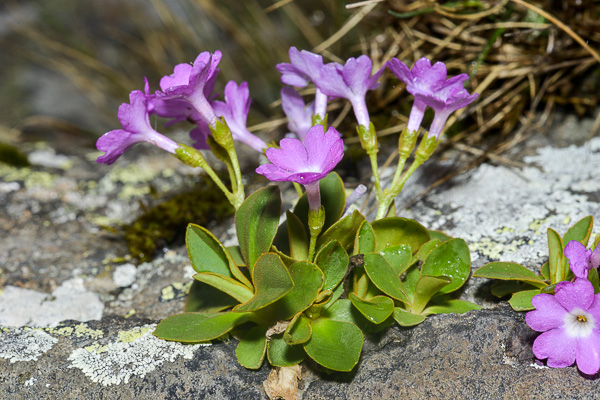
\includegraphics[scale=3]{fig/primulapedemontana_7.jpg}
%	\caption{reference de la photo}
%	\label{frontpage}
%\end{center}
%\end{figure}

%\textit{Primula pedemontana} Crédit photo : Florian Boucher
\end{frame}


\begin{frame} 
\frametitle{There Is No Largest Prime Number} 
\framesubtitle{The proof uses \textit{reductio ad absurdum}.} 
\begin{theorem}
There is no largest prime number. \end{theorem} 
\begin{enumerate} 
\item<1-| alert@1> Suppose $p$ were the largest prime number. 
\item<2-> Let $q$ be the product of the first $p$ numbers. 
\item<3-> Then $q+1$ is not divisible by any of them. 
\item<1-> But $q + 1$ is greater than $1$, thus divisible by some prime
number not in the first $p$ numbers.
\end{enumerate}
\end{frame}

\begin{frame}{A longer title}

\end{frame}

\begin{frame}[fragile]
\begin{lstlisting}
  tadaaa = function(fame = 9000, class = "hero"){
  #et ouai ca marche ma gueule
  print("youpi")}
\end{lstlisting}
\end{frame}
  

\cite{}
\bibliographystyle{authordate1}
\bibliography{Primula}

\end{document}